\documentclass[doc/report.tex]{subfiles}

% Present the details of your experiments and their results.

\newcommand{\err}{\cellcolor{red!25}}

\begin{document}

\section{Experiments and Results}
% TODO intro

\subsection{Feature Extraction from Pretrained AlexNet}
Table 1 describes the performance of various classifers that were trained based
on the features extracted from the last fully connected layer (FC8) of the
AlexNet and the last pooling layers of ResNet18 and ResNet50. Image
Augmnetation techniques such as translation and rotation seemed to be having a
negative impact on the perfromance of these classifers and hence were not
included in the results.

\begin{table}[h]
\centering
\caption{Accuracy of various trained classifers}
\label{tab:my-table1}
\begin{tabular}{|l|c|c|}
\hline
\multicolumn{1}{|c|}{Pre-Trained Model} & Classifier                                 & Accuracy \\ \hline
AlexNet                                 & SVM                                        & 99.04\%  \\ \hline
AlexNet                                 & KNN                                        & 98.39\%  \\ \hline
AlexNet                                 & Naïve Bayes                                & 98.39\%  \\ \hline
AlexNet                                 & Discriminant Analysis                      & 99.22\%  \\ \hline
ResNet18                                & SVM                                        & 99.83\%  \\ \hline
ResNet18                                & KNN                                        & 99.57\%  \\ \hline
ResNet18                                & Naïve Bayes                                & 99.00\%  \\ \hline
ResNet18                                & Discriminant Analysis                      & 99.83\%  \\ \hline
ResNet50                                & SVM                                        & 99.96\%  \\ \hline
ResNet50                                & KNN                                        & 99.76\%  \\ \hline
ResNet50                                & Naïve Bayes                                & 99.26\%  \\ \hline
ResNet50                                & \multicolumn{1}{l|}{Discriminant Analysis} & 99.87\%  \\ \hline
\end{tabular}%
\end{table}

\subsection{Retraining the pretrained AlexNet}
The transfer learning model was trained over the training image datset using
MATLAB 2018b on a Windows 10 Operating System on a single core i3 CPU with 8GB
of RAM. While the initial results from the trained classier were promising, by
means of training data augmentation and optimization of the training parameters
we are able to acheive a very accurate classifier while also reducing the
training time by half. Table 2 depicts the effect of training parameters on the
classifeir performance. 

\begin{table}[h]
\centering
\caption{Training Parameter Analysis}
\label{tab:my-table2}
\resizebox{\textwidth}{!}{%
\begin{tabular}{|c|c|c|c|c|c|c|c|c|}
\hline
\# & LR & Epochs & Batch Size & LR Drop Period & LR Drop Factor & Validation Accuracy & Test Accuracy & Time \\ \hline
1 & 0.0005 & 8 & 512 & 2 & 0.9 & 92.83\% & 93.57\% & 22 min \\ \hline
2 & 0.0005 & 8 & 256 & 2 & 0.9 & 92.61\% & 93.91\% & 22min  \\ \hline
3 & 0.0005 & 8 & 128 & 2 & 0.9 & 96.20\% & 97.39\% & 25min  \\ \hline
4 & 0.0005 & 8 & 128 & 2 & 0.6 & 97.50\% & 97.96\% & 25min  \\ \hline
5 & 0.0005 & 4 & 128 & 2 & 0.6 & 95.54\% & 95.48\% & 13min  \\ \hline
6 & 0.0001 & 4 & 128 & 2 & 0.6 & 98.91\% & 99.04\% & 13min  \\ \hline
7 & 0.0001 & 4 & 128 & 1 & 0.6 & 99.35\% & 99.09\% & 12min  \\ \hline
\end{tabular}%
}
\end{table}

\subsection{Experiments with self-organizing map}
A classifier using SOM was implemented and tested with different features.  The
results are shown in table \ref{tbl:som}. LBP $W$x$H$/$n$ means that the images
were resized to WxH and then split into $n\times n$ cells. The tiles produced
by the SOM using the AlexNet and LBP 100x100/16 are shown in figure
\ref{fig:som_tiles}. The time shown is the total time to train and evaluate the
classifier. It may vary for different computers but it gives a rough estimate
of how computation intensive each setup is in comparison to each other.
    
\begin{table}[h]
    \centering
    \begin{tabular}{lrlrr}
        features & feature count & classifier & time (minutes) & accuracy \\\hline
        AlexNet & 4096 & SOM 8x8 & 15 & 98\% \\
        LBP 100x100/10 + SURF & 6400 & SOM 8x8 & ?? & 80\% \\
        LBP 100x100/16 & 2891 & SOM 16x16 & 40 & 75\% \\
        LBP 100x100/10 & 5900 & SOM 8x8 & 32 & 74\% \\
        SURF & 500 & SOM 8x8 & 55 & 74\% \\
        LBP 100x100/16 & 2891 & SOM 8x8 & 20 & 73\% \\
        LBP 100x100/16 & 2891 & SOM 32x32 & 240 & 73\% \\
        LBP 100x100/16 & 2891 & SOM 6x6 & 7 & 69\% \\
        LBP 100x100/16 & 2891 & SOM 4x4 & 4 & 63\% \\
        grayscale 100x100 & 10000 & SOM 8x8 & 40 & 60\% \\
    \end{tabular}%
    \caption{Result of experiments, sorted by accuracy.}
    \label{tbl:som}
\end{table}

\begin{figure}[h]
    \centering
    \begin{subfigure}[t]{0.9\textwidth}
        \centering
        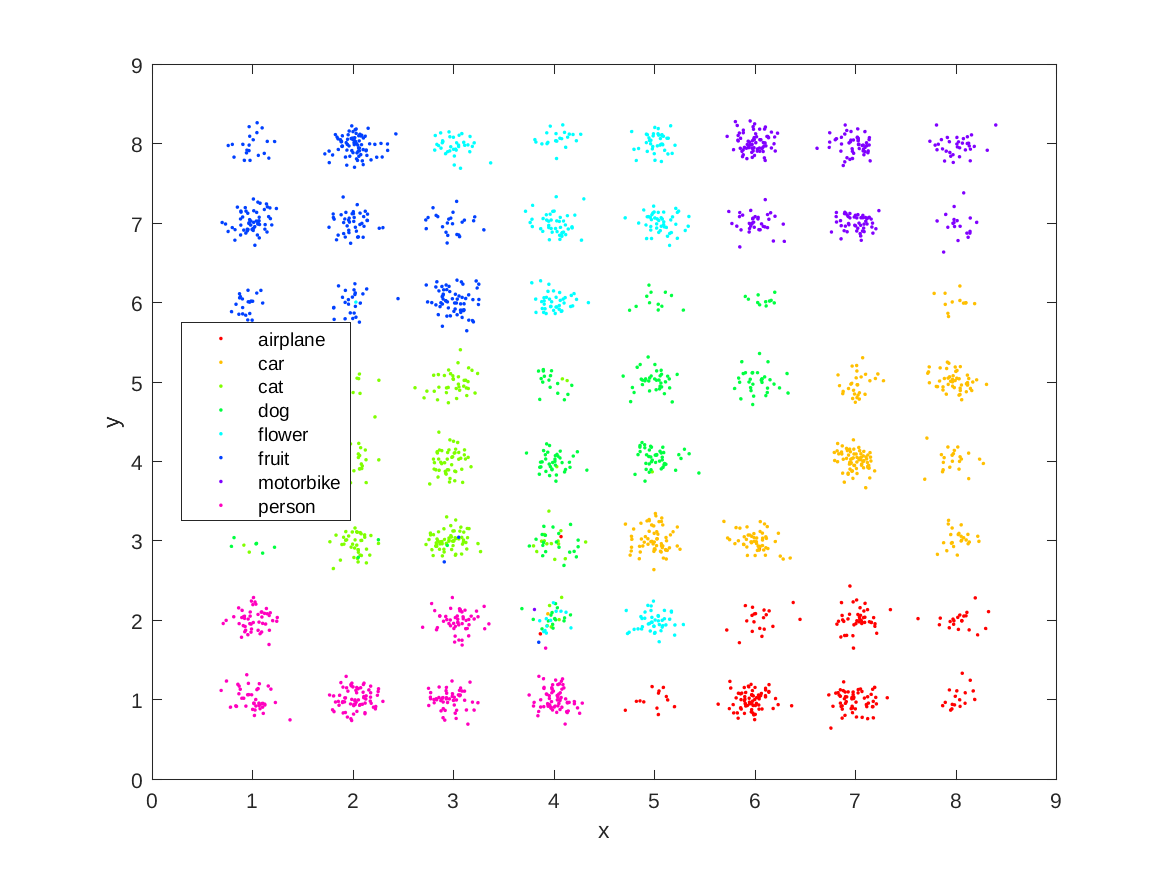
\includegraphics[width=\textwidth]{doc/fig/som_alex.png}
        \caption{AlexNet.}
    \end{subfigure}

    \begin{subfigure}[t]{0.9\textwidth}
        \centering
        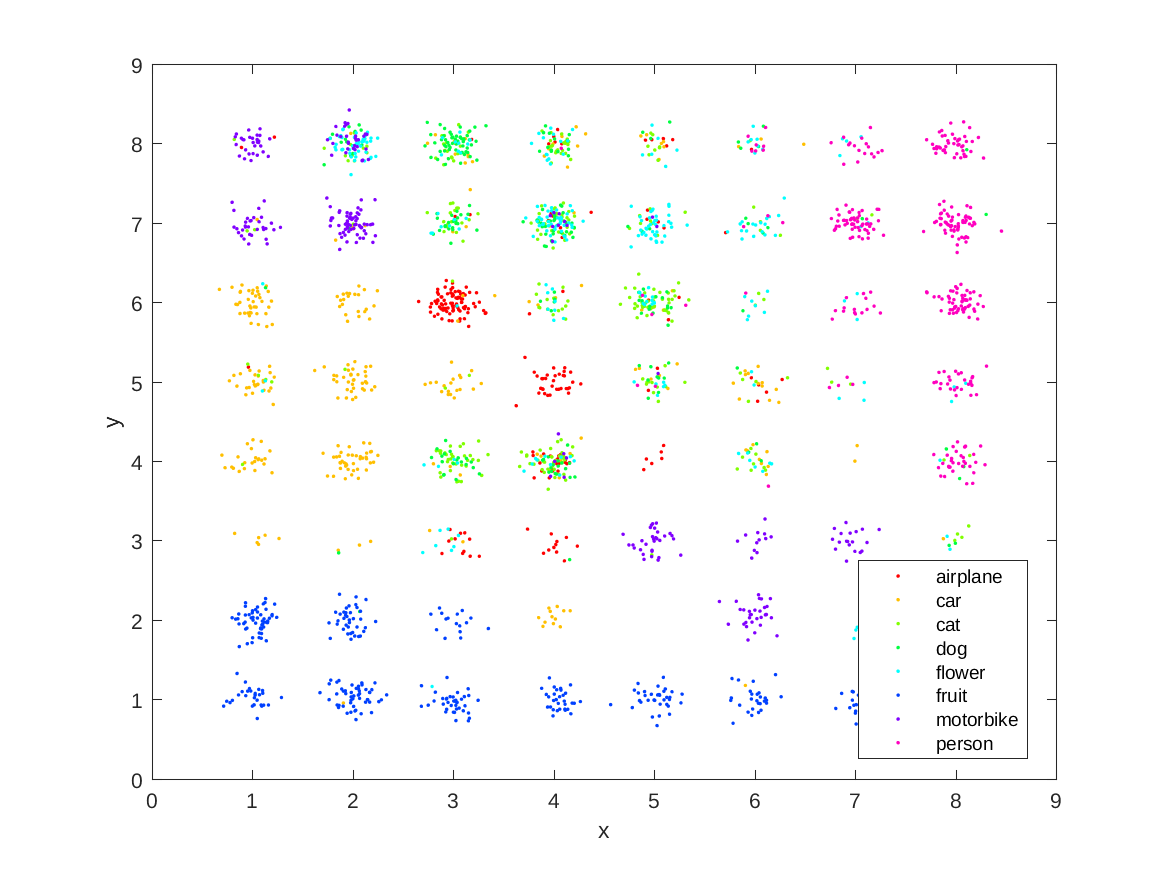
\includegraphics[width=\textwidth]{doc/fig/som_lbp.png}
        \caption{LBP 100x100/16}
    \end{subfigure}%
    \caption{Test dataset plotted at tile location as predicted by classifier.}
    \label{fig:som_tiles}
\end{figure}

\subsubsection{Sample test}
A very small sample test with 21 self taken photos were also tested using the
SOM classifier with AlexNet features. The images were however not cropped like
the training set as they were simply taken directly from a photo library. The
classifications are listed in table \ref{tbl:sample}. 76\% of the pictures were
classified correctly. Two of the cats that were outside in the grass were
incorrectly classified as flowers. Two of the dogs were also classified as
flowers but were inside and nothing green or colorful. A photo taken of a
person from the side was classified as a dog.
    
\begin{table}[h]
    \centering
    \begin{tabular}{ll}
        object in photo & predicted object \\\hline
        cat 1       & cat \\
        cat 2       & \err flower \\
        cat 3       & cat \\
        cat 4       & cat \\
        cat 5       & cat \\
        cat 6       & \err flower \\
        cat 7       & cat \\
        cat 8       & cat \\
        cat 9       & cat \\
        cat 10      & cat \\
        dog 1       & dog \\
        dog 2       & \err flower \\
        dog 3       & \err flower \\
        flower 1    & flower \\
        person 1    & person \\
        person 2    & \err dog \\
        person 3    & person \\
        person 4    & person \\
        person 5    & person \\
        person 6    & person \\
        person 7    & person \\
    \end{tabular}%
    \caption{Classifications of a small independent test sample.}
    \label{tbl:sample}
\end{table}


\end{document}
